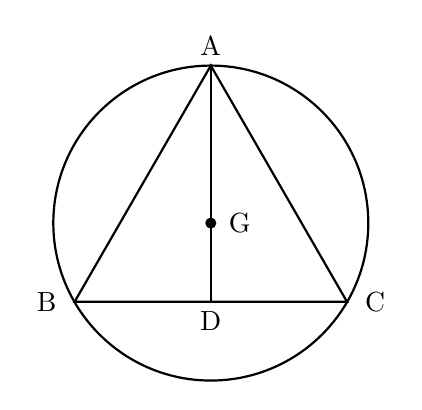
\begin{tikzpicture}[scale=1]

    % Draw the circle centered at (0,0.3) to align with G
    % Radius is set to 2 units
    \draw[thick] (0,0.3) circle (2cm);

    % Coordinates for the points based on visual proportions
    \coordinate (A) at (0,2.3);    % Top vertex on the circle
    \coordinate (B) at (-1.73,-0.7); % Bottom-left vertex on the circle
    \coordinate (C) at (1.73,-0.7);  % Bottom-right vertex on the circle
    \coordinate (D) at (0,-0.7);     % Midpoint of BC
    \coordinate (G) at (0,0.3);      % Point G on the segment AD (center of circle)

    % Draw the triangle ABC
    \draw[thick] (A) -- (B) -- (C) -- cycle;

    % Draw the vertical segment AD
    \draw[thick] (A) -- (D);

    % Draw the point dot for G
    \fill (G) circle (2pt);

    % Labels for the points
    % Placed exactly as they appear in the provided image
    \node[above] at (A) {A};
    \node[left=3pt] at (B) {B};
    \node[right=3pt] at (C) {C};
    \node[right=3pt] at (G) {G};
    \node[below] at (D) {D};

\end{tikzpicture}